\documentclass[10pt,a4paper]{article}
\usepackage[utf8]{inputenc}

% \usepackage{ngerman}  % german documents
\usepackage{graphicx}  % import graphics einbinden
\usepackage{listings}  % support source code listing
\usepackage{amsmath}  % math stuff
\usepackage{amssymb} % 
\usepackage{a4wide} % wide pages
\usepackage{fancyhdr} % nice headers
\usepackage{float}
\usepackage{longtable}
\usepackage{xcolor}
\usepackage{booktabs}
\definecolor{darkpastelgreen}{rgb}{0.01, 0.75, 0.24}
\definecolor{spirodiscoball}{rgb}{0.06, 0.75, 0.99}
\definecolor{smalt}{rgb}{0.0, 0.2, 0.6}
\definecolor{armygreen}{rgb}{0.29, 0.33, 0.13}
\definecolor{awesome}{rgb}{1.0, 0.13, 0.32}
\definecolor{bittersweet}{rgb}{1.0, 0.44, 0.37}
\definecolor{bananayellow}{rgb}{1.0, 0.88, 0.21}
\definecolor{blue}{rgb}{0.0, 0.0, 1.0}
\definecolor{red}{rgb}{1.0, 0.0, 0.0}
\definecolor{green}{rgb}{0.0, 1.0, 0.0}



\lstset{basicstyle=\footnotesize,language=Python,breaklines=true,numbers=left, numberstyle=\tiny, stepnumber=5,firstnumber=0, numbersep=5pt} % set up listings
\pagestyle{fancy}             % header
\setlength{\parindent}{0pt}   % no indentation
 

\usepackage[pdfpagemode=None, colorlinks=true,  % url coloring
           linkcolor=blue, urlcolor=blue, citecolor=blue, plainpages=false, 
           pdfpagelabels,unicode]{hyperref}
           
% change enums style: first level (a), (b), (c)           
\renewcommand{\labelenumi}{(\alph{enumi})}
\renewcommand{\labelenumii}{(\arabic{enumii})}

\newcommand{\norm}[1]{\left\lVert#1\right\rVert}

%lecture name
\newcommand{\lecture}{
	Bioinformatics III
}           

%assignment iteration
\newcommand{\assignment}{
	Fifth Assignment
}


%set up names, matricle number, and email
\newcommand{\authors}{
  \begin{tabular}{rl}
    \href{mailto:s8tbscho@stud.uni-saarland.de}{Thibault Schowing} & (2571837)\\
    \href{mailto:wiebkeschmitt@outlook.de}{Wiebke Schmitt} & (2543675)
  \end{tabular}
}

% use to start a new exercise
\newcommand{\exercise}[1]
{
  \stepcounter{subsection}
  \subsection*{Exercise \thesubsection: #1}

}

\begin{document}
\title{\Large \lecture \\ \textbf{\normalsize \assignment}}
\author{\authors}

\setlength \headheight{25pt}
\fancyhead[R]{\begin{tabular}{r}\lecture \\ \assignment \end{tabular}}
\fancyhead[L]{\authors}


\setcounter{section}{5} % modify for later sheets, i.e. 2, 3, ...
%\section{Introduction to Python and some Network Properties} % optional, note that section invocation sets the section counter + 1, so adapt the setcounter command
\maketitle

%WIEBKE !!! READ THIS !!! 
% Usefull with Latex and maths: a list of the symbols ! https://reu.dimacs.rutgers.edu/Symbols.pdf

%EXERCICE 1
\exercise{Cliques and Network Evolution}
\begin{enumerate}

% A
\item \textit{Reading network files}\\ 
The class GenericNetwork contains the functions to read the network from a file and also the function to count cliques.

\lstinputlisting[label=lst-1, caption={generic\textunderscore network.py}] {../Scripts/generic\string_network.py}



% B
\newpage
\item \textit{Finding Cliques}\\

The function to find cliques of n nodes in a network is in the class generic\textunderscore network.py in listing \ref{lst-1}. This function returns the list of cliques of size n. In the main program (listing \ref{lst-2}), the function \textit{remove\textunderscore contained\textunderscore cliques} remove the smaller cliques contained in the bigger one as requested. \textbf{The code seems to work, but the execution time is too long.} We are aware that this is not the optimal solution. 




% C
\item \textit{Evolving Network}\\

In the listing \ref{lst-2}, the main program is executed and different functions are implemented. The function evolve takes a network and a number of time steps and randomly remove or add edges in the network. 

\lstinputlisting[label=lst-2, caption={main5.py}] {../Scripts/main5.py}



% D
\newpage
\item \textit{Cliques in evolving networks.}
Due to the execution time, this has been run on a minimized version of the rat network.

\begin{figure}[H]
	\centering
	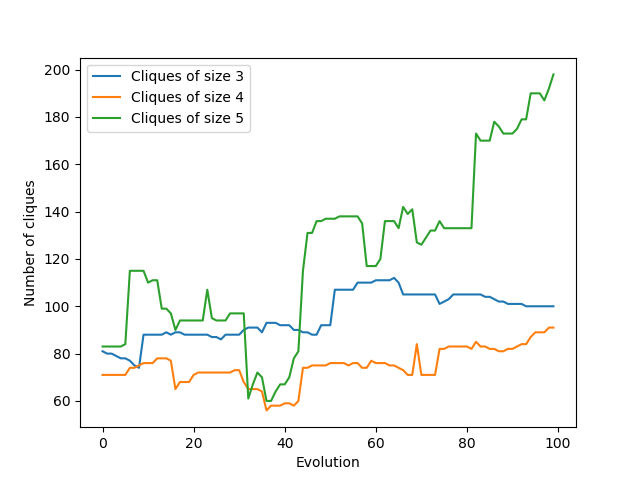
\includegraphics[width=0.7\linewidth]{img/100randomMiniRat}
	\caption{Evolution of the number of cliques during 100 randomization steps on a randomly minimized version of the rat network. }
	\label{fig:100randomminirat}
\end{figure}



% E
\item \textit{Randomizing Network}
The class \textit{randomized\textunderscore network} builds a randomized network. Randomizing a network this way, keep its degree (number of edges) the same but change the topological structure of the graph. According to the Wikipedia definition of Degree-preserving randomization: "\textit{Degree Preserving Randomization is a technique used in Network Science that aims to assess whether or not variations observed in a given graph could simply be an artifact of the graph's inherent structural properties rather than properties unique to the nodes, in an observed network.} "(\url{https://en.wikipedia.org/wiki/Degree-preserving_randomization}, Mai 2018). In other words, we use the randomization to verify whether the topology of the original graph is due to randomness or has a specific structure. \\



\lstinputlisting[label=lst-2, caption={randomized\textunderscore network.py}] {../Scripts/randomized\string_network.py}



% F
\newpage
\item \textit{Examining motif enrichment}\\
Please be aware that the function to extract the cliques is still not optimal here. 




\end{enumerate}










% NEW EXERCICE
\newpage
\exercise{Annotations in Protein–Protein–Interaction Networks}
\begin{enumerate}
	
	% A
	\item \textbf{Adding annotations to PPI-networks}\\
	
		%TODO listing at the end
		The listings for this exercise are at the end of the document.

		%\lstinputlisting[label=lst-1, caption={layout\string_main.py}] {../Scripts/layout\string_main.py}

	\item \textbf{Generating an overview}\\
	
	
	
	
	
	
	For Chicken: 
	
	\begin{table}[H]
		\centering
		\caption{Chicken network overview}
		\vspace*{1mm}
		\label{chickentableoverview}
		\begin{tabular}{llllll}
			\hline
			\multicolumn{1}{|l|}{Interactions in the network}     & \multicolumn{1}{l|}{300} & \multicolumn{1}{l|}{}                           & \multicolumn{1}{l|}{}    & \multicolumn{1}{l|}{}               & \multicolumn{1}{l|}{}     \\ \hline
			\multicolumn{1}{|l|}{Proteins in the network}         & \multicolumn{1}{l|}{281} & \multicolumn{1}{l|}{Protein without annotation} & \multicolumn{1}{l|}{44}  & \multicolumn{1}{l|}{Percentage}     & \multicolumn{1}{l|}{15.6} \\ \hline
			\multicolumn{1}{|l|}{\textbf{Annotation per protein}} & \multicolumn{1}{l|}{}    & \multicolumn{1}{l|}{}                           & \multicolumn{1}{l|}{}    & \multicolumn{1}{l|}{}               & \multicolumn{1}{l|}{}     \\ \hline
			\multicolumn{1}{|l|}{Smallest number}                 & \multicolumn{1}{l|}{0}   & \multicolumn{1}{l|}{Average number}             & \multicolumn{1}{l|}{7.7} & \multicolumn{1}{l|}{Biggest number} & \multicolumn{1}{l|}{88}   \\ \hline
			\multicolumn{1}{|l|}{\textbf{Protein per annotation}} & \multicolumn{1}{l|}{}    & \multicolumn{1}{l|}{}                           & \multicolumn{1}{l|}{}    & \multicolumn{1}{l|}{}               & \multicolumn{1}{l|}{}     \\ \hline
			\multicolumn{1}{|l|}{Smallest number}                 & \multicolumn{1}{l|}{1}   & \multicolumn{1}{l|}{Average number}             & \multicolumn{1}{l|}{1.55} & \multicolumn{1}{l|}{Biggest number} & \multicolumn{1}{l|}{27}  \\ \hline
			&                          &                                                 &                          &                                     &                          
		\end{tabular}
	\end{table}

	For pig: 
	
	\begin{table}[H]
		\centering
		\caption{Pig network overview}
		\vspace*{1mm}
		\label{pignetworkoverview}
		\begin{tabular}{llllll}
			\hline
			\multicolumn{1}{|l|}{Interactions in the network}     & \multicolumn{1}{l|}{50} & \multicolumn{1}{l|}{}                           & \multicolumn{1}{l|}{}    & \multicolumn{1}{l|}{}               & \multicolumn{1}{l|}{}     \\ \hline
			\multicolumn{1}{|l|}{Proteins in the network}         & \multicolumn{1}{l|}{51} & \multicolumn{1}{l|}{Protein without annotation} & \multicolumn{1}{l|}{13}  & \multicolumn{1}{l|}{Percentage}     & \multicolumn{1}{l|}{25.5} \\ \hline
			\multicolumn{1}{|l|}{\textbf{Annotation per protein}} & \multicolumn{1}{l|}{}   & \multicolumn{1}{l|}{}                           & \multicolumn{1}{l|}{}    & \multicolumn{1}{l|}{}               & \multicolumn{1}{l|}{}     \\ \hline
			\multicolumn{1}{|l|}{Smallest number}                 & \multicolumn{1}{l|}{0}  & \multicolumn{1}{l|}{Average number}             & \multicolumn{1}{l|}{5.5} & \multicolumn{1}{l|}{Biggest number} & \multicolumn{1}{l|}{40}   \\ \hline
			\multicolumn{1}{|l|}{\textbf{Protein per annotation}} & \multicolumn{1}{l|}{}   & \multicolumn{1}{l|}{}                           & \multicolumn{1}{l|}{}    & \multicolumn{1}{l|}{}               & \multicolumn{1}{l|}{}     \\ \hline
			\multicolumn{1}{|l|}{Smallest number}                 & \multicolumn{1}{l|}{1}  & \multicolumn{1}{l|}{Average number}             & \multicolumn{1}{l|}{1.13} & \multicolumn{1}{l|}{Biggest number} & \multicolumn{1}{l|}{5} \\ \hline
			&                         &                                                 &                          &                                     &                          
		\end{tabular}
	\end{table}
	
	
	for Human: 
	
	
	\begin{table}[H]
		\centering
		\caption{Human network overview}
		\vspace*{1mm}
		\label{humanoverview}
		\begin{tabular}{llllll}
			\hline
			\multicolumn{1}{|l|}{Interactions in the network}     & \multicolumn{1}{l|}{275472} & \multicolumn{1}{l|}{}                           & \multicolumn{1}{l|}{}      & \multicolumn{1}{l|}{}               & \multicolumn{1}{l|}{}     \\ \hline
			\multicolumn{1}{|l|}{Proteins in the network}         & \multicolumn{1}{l|}{17087}  & \multicolumn{1}{l|}{Protein without annotation} & \multicolumn{1}{l|}{2262}  & \multicolumn{1}{l|}{Percentage}     & \multicolumn{1}{l|}{13.2} \\ \hline
			\multicolumn{1}{|l|}{\textbf{Annotation per protein}} & \multicolumn{1}{l|}{}       & \multicolumn{1}{l|}{}                           & \multicolumn{1}{l|}{}      & \multicolumn{1}{l|}{}               & \multicolumn{1}{l|}{}     \\ \hline
			\multicolumn{1}{|l|}{Smallest number}                 & \multicolumn{1}{l|}{0}      & \multicolumn{1}{l|}{Average number}             & \multicolumn{1}{l|}{7.22}  & \multicolumn{1}{l|}{Biggest number} & \multicolumn{1}{l|}{184}  \\ \hline
			\multicolumn{1}{|l|}{\textbf{Protein per annotation}} & \multicolumn{1}{l|}{}       & \multicolumn{1}{l|}{}                           & \multicolumn{1}{l|}{}      & \multicolumn{1}{l|}{}               & \multicolumn{1}{l|}{}     \\ \hline
			\multicolumn{1}{|l|}{Smallest number}                 & \multicolumn{1}{l|}{1}      & \multicolumn{1}{l|}{Average number}             & \multicolumn{1}{l|}{10.6} & \multicolumn{1}{l|}{Biggest number} & \multicolumn{1}{l|}{1554} \\ \hline
			&                             &                                                 &                            &                                     &                          
		\end{tabular}
	\end{table}

	\newpage
	\item \textbf{Examining the most/least common annotations}\textit{Implement a function that returns
		the n most common and n least common GO identifiers in a given annotated network. If
		there are several GO identifiers that are associated with the same number of proteins, choose
		the ones with the lower lexicographical order first.
}
	
	
	
	
		% Please add the following required packages to your document preamble:
		% \usepackage{booktabs}
		% \usepackage{graphicx}
		\begin{table}[H]
			\centering
			\caption{Function of the 5 most common GO identifiers of the human network. }
			\vspace*{1mm}
			\label{my-label}
				\begin{tabular}{|l|l|l|}
					\hline
					\textbf{GO id} & \textbf{Quantity} & \textbf{Biological Process}                                                                                                                                           \\ \hline
					GO:0006351     & 1562              & The cellular synthesis of RNA on a template of DNA.                                                                                                                   \\ \hline
					GO:0045944     & 1029              & \begin{tabular}[c]{@{}l@{}}Any process that activates or increases the frequency, \\ rate or extent of transcription from an RNA polymerase II promoter.\end{tabular} \\ \hline
					GO:0007165     & 1010              & Signal transduction                                                                                                                                                   \\ \hline
					GO:0006357     & 960               & \begin{tabular}[c]{@{}l@{}}Any process that modulates the frequency, rate or extent \\ of transcription mediated by RNA polymerase II.\end{tabular}                   \\ \hline
					GO:0006355     & 765               & \begin{tabular}[c]{@{}l@{}}Any process that modulates the frequency, rate or extent \\ of cellular DNA-templated transcription\end{tabular}                           \\ \hline
				\end{tabular}
		\end{table}
	
	We can observe that these annotations concerns general process happening almost in every cell. This explains why they are the most common in opposition as the annotations in the table below, which concerns specific reaction or process concerning particular location or molecules. 
	
	
	
	\begin{table}[H]
		\centering
		\caption{Function of the 5 least common GO identifiers of the human network}
		\vspace*{1mm}
		\label{my-label}
		\begin{tabular}{|l|l|l|}
			\hline
			\textbf{GO id} & \textbf{Quantity} & \textbf{Biological Process}                 \\ \hline
			GO:0000003     & 1                 & Reproduction                                \\ \hline
			GO:0000011     & 1                 & Vacuole inheritance                         \\ \hline
			GO:0000032     & 1                 & Cell wall mannoprotein biosynthetic process \\ \hline
			GO:0000053     & 1                 & Argininosuccinate metabolic process         \\ \hline
			GO:0000097     & 1                 & Sulfur amino acid biosynthetic process      \\ \hline
		\end{tabular}
	\end{table}

	
	%d
	\newpage
	\item \textbf{Investigating annotation enrichment}\textit{The hypergeometric distribution can be used to
		find out if a given annotation is significantly overrepresented in interacting compared to
		non–interacting protein pairs. Implement a function that computes pA for every annotation A in a given annotated network.}
	
	
	\begin{table}[H]
		\centering
		\caption{Number and percentage of annotation with certain p-value}
		\vspace*{1mm}
		\label{my-penis}
		\begin{tabular}{|l|l|l|}
			\hline
		p-value	& Number & Percentage \\ \hline
			p \textless 0.05    &   35     &     2.721\%       \\ \hline
			p \textgreater 0.5  &   43     &     3.343\%       \\ \hline
			p \textgreater 0.95 &   1243     &   96.656\%         \\ \hline
		\end{tabular}
	\end{table}

	
	
	\begin{table}[H]
		\centering
		\caption{Annotations with the \textbf{five lowest} $pA$ and \textbf{five highest} $pA$  }
		\label{my-label}
		\begin{tabular}{|l|l|l|l|l|}
			\hline
			\textbf{GO:ID }     & \textbf{pA}  & \textbf{Nb Protein} & \begin{tabular}[c]{@{}l@{}}\textbf{Nb Interact.} \\ \textbf{protein}\end{tabular} & \textbf{Annotation}   \\ \hline
			GO:0009409 & 4.3907e-07  & 3 &    3     & Response to cold   \\ \hline
			GO:0030154 & 1.7908e-05  & 7 &    4     & Cell differentiation   \\ \hline
			GO:0007169 & 0.0002 & 3 &    2     & \begin{tabular}[c]{@{}l@{}}Transmembrane receptor protein\\ tyrosine kinase signaling pathway\end{tabular} \\ \hline
			GO:0000712 & 0.0002 & 3 &    2     & \begin{tabular}[c]{@{}l@{}}Resolution of meiotic recombination\\ intermediates\end{tabular}                \\ \hline
			GO:0032570 & 0.0002 & 3 &    2     & Response to progesterone   \\ \hline
			\hline
			GO:0007049 & 1                      & 10 &    0    & Cell cycle  \\ \hline
			GO:0006096 & 1                      & 9  &    0    & Glycotic process     \\ \hline
			GO:0055114 & 1                      & 9  &    0    & Oxydation-reduction process    \\ \hline
			GO:0006457 & 1                      & 9  &    0    & Protein folding    \\ \hline
			GO:0006094 & 1                      & 8  &    0    & Gluconeogenesis  \\ \hline
		\end{tabular}
	\end{table}
	
	
	%TODO comment and answer question
	TODO
	
	The closer the p-value to zero, the more significant the GO term associated with the group of protein is. The five GO term with the lowest p-value describe very specific process in opposition to the ones with the five highest p-value.
	
	\textit{Are interacting proteins functionally more similar than non–interacting protein ?}\\
	???????   No real similarity between the interacting protein and the non-interacting. 
	
	\textit{Was this to be expected? Why (not)?}
	
	%e
	\newpage
	\item \textbf{e) Investigating annotation combinations}\textit{s: Implement a function that computes if certain
		annotation combinations occur more frequently than expected. The function should take
		the combination size k and the number of random distributions r. Additionally, let n be the
		number of proteins in the network and nA the number of proteins with annotation}
	
	
	
	\begin{table}[H]
		\centering
		\caption{Number and percentage of combination with certain p-value}
		\vspace*{1mm}
		\label{my-penis2}
		\begin{tabular}{|l|l|l|}
			\hline
			p-value	& Number & Percentage \\ \hline
			p \textless 0.05    &   9794     &     49.25\%       \\ \hline
			p \textgreater 0.5  &   0        &       0.0\%       \\ \hline
			p \textgreater 0.95 &   1252     &     6.295\%      \\ \hline
		\end{tabular}
	\end{table}


	\begin{table}[H]
		\centering
		\caption{The m combinations with the smallest pc and the m combinations with the highest pc}
		\vspace*{1mm}
		\label{penis-label}
		\begin{tabular}{|l|llll}
			\cline{1-1}
			Three smallest Pc:                                                    &                                &                              &                                                                                                          &                                                                                                          \\ \hline
			GO:IDs                                                                & \multicolumn{1}{l|}{Occurence} & \multicolumn{1}{l|}{p-Value} & \multicolumn{1}{l|}{Annotation 1}                                                                        & \multicolumn{1}{l|}{Annotation 2}                                                                        \\ \hline
			\begin{tabular}[c]{@{}l@{}}'GO:0006897', \\ 'GO:0006898'\end{tabular} & \multicolumn{1}{l|}{1}         & \multicolumn{1}{l|}{0.0}     & \multicolumn{1}{l|}{endocytosis}                                                                         & \multicolumn{1}{l|}{\begin{tabular}[c]{@{}l@{}}Receptor-mediated\\ endocytosis\end{tabular}}             \\ \hline
			\begin{tabular}[c]{@{}l@{}}'GO:0006898', \\ 'GO:0021517'\end{tabular} & \multicolumn{1}{l|}{2}         & \multicolumn{1}{l|}{0.0}     & \multicolumn{1}{l|}{\begin{tabular}[c]{@{}l@{}}Receptor-mediated\\ endocytosis\end{tabular}}             & \multicolumn{1}{l|}{\begin{tabular}[c]{@{}l@{}}Ventral spinal cord\\ development\end{tabular}}           \\ \hline
			\begin{tabular}[c]{@{}l@{}}'GO:0008203', \\ 'GO:0048813'\end{tabular} & \multicolumn{1}{l|}{1}         & \multicolumn{1}{l|}{0.0}     & \multicolumn{1}{l|}{\begin{tabular}[c]{@{}l@{}}Cholesterole metabolism\\ process\end{tabular}}           & \multicolumn{1}{l|}{\begin{tabular}[c]{@{}l@{}}Dendrites \\ morphogenesis\end{tabular}}                  \\ \hline\hline
			Three biggest Pc:                                                     &                                &                              &                                                                                                          &                                                                                                          \\ \hline 
			\begin{tabular}[c]{@{}l@{}}'GO:0006355', \\ 'GO:0006355'\end{tabular} & \multicolumn{1}{l|}{1}         & \multicolumn{1}{l|}{0.71}    & \multicolumn{1}{l|}{\begin{tabular}[c]{@{}l@{}}Regulation of transcription\\ DNA-templated\end{tabular}} & \multicolumn{1}{l|}{\begin{tabular}[c]{@{}l@{}}Regulation of transcription\\ DNA-templated\end{tabular}} \\ \hline
			\begin{tabular}[c]{@{}l@{}}'GO:0006351', \\ 'GO:0050821'\end{tabular} & \multicolumn{1}{l|}{1}         & \multicolumn{1}{l|}{0.71}    & \multicolumn{1}{l|}{\begin{tabular}[c]{@{}l@{}}Transcription\\ DNA-templated\end{tabular}}               & \multicolumn{1}{l|}{Protein stabilization}                                                               \\ \hline
			\begin{tabular}[c]{@{}l@{}}'GO:0006351', \\ 'GO:0043066'\end{tabular} & \multicolumn{1}{l|}{1}         & \multicolumn{1}{l|}{0.69}    & \multicolumn{1}{l|}{\begin{tabular}[c]{@{}l@{}}Transcription\\ DNA-templated\end{tabular}}               & \multicolumn{1}{l|}{\begin{tabular}[c]{@{}l@{}}Negative regulation of\\ apoptotic process\end{tabular}}  \\ \hline
		\end{tabular}
	\end{table}
	
	
	%TODO Briefly comment the results
	TODO - COMMENT
	
	\newpage
	\item Listings:
	
	\lstinputlisting[label=lst-1, caption={task52\textunderscore main.py}] {../Scripts/task52\string_main.py}
	\newpage
	\lstinputlisting[label=lst-1, caption={UniprotReader.py}] {../Scripts/UniprotReader.py}
	\newpage
	\lstinputlisting[label=lst-1, caption={GOreader.py}] {../Scripts/GOreader.py}
	\newpage
	\lstinputlisting[label=lst-1, caption={annotated\textunderscore network.py}] {../Scripts/annotated\string_network.py}
	
	
	
	
\end{enumerate}

\end{document}